\documentclass{article}
\usepackage[colorlinks=true,linkcolor=black,urlcolor=blue]{hyperref} %% links
\usepackage{graphicx}

\title{SETAP}
\author{Names go here}
\begin{document}
\maketitle
\tableofcontents
\newpage
\section{Introduction}%
\label{sec:intro}
We are making a top down 2d survival game.

\section{Problem Specification}%
\label{sec:problem}
\subsection{Eliciting requirements}%
\label{subsec:reqs}
To elicit requirements we have used interviews and questionnaires. Our target age group is that of
people 15 years to 30 years old. This is because this reflects the demographic
of people who play games within this genre. Of course while people outside of
this group can play the game. The likelyhood of them doing so is lesser

Our interviews were a discussion with 9 people. these ranged in age from 15 to
21. People had the abiliy to discuss within the answers and expand on their
views even if it was not fully related.
our questions were
\begin{enumerate}
	\item What kind of games do you play?
	\item What are your thoughts on open-world games?
	\item What platform do you play games on?
	\item If you play games for an end goal, what kind of end goal are you looking for?
	\item Are you more into singleplayer or multiplayer games?
	\item What features do you like in the games you play?
\end{enumerate}

%% TODO: add in the interviews
\subsection{Requirements}%
\label{subsec:ureqs}
These requirements are garnered from our interviews. Our main line is our user
requirements with each of them broken down into a set of system requirements.

These are ordered in the priority of these tasks. The first ones being the most
important, the latter being the least. This is both for the user requirements
and the system requirements within them.

%% This level of detail good
%% TODO: update all of them to reflect this kind of detail
\paragraph{Users should be able to explore a procedurally generated map.}
\begin{itemize}
	\item The map size will be 100 x 100 and include 10,000 tiles in total.
	\item Each tile should be able to carry 1 item and character (user or NPC).
	\item The player will move by moving from tile to tile.
	\item Users will spawn in the middle of the map at point (50, 50).
	\item The map will be modelled as an object.
\end{itemize}

\paragraph{ Users should be able to interact with NPCs.}
\begin{itemize}
	\item Interactions will be both hostile and passive depending on the type of NPC.
	\item Each NPC will be modelled as an object that interacts with the user.
	\item NPCs will drop items when killed, which the user should be able to collect.
	\item There will be passive NPCs that can sell you stuff using a bartering system.
\end{itemize}

\paragraph{Users should be able to save their progress into a save file.}
\begin{itemize}
	\item The file should store the world map as a 2D array.
	\item The file should store the user’s current inventory and that of any chests they have placed.
	\item The file should store the user’s position and the position of any spawned NPCs or items.
	\item The file should store the user’s current points acquired and stats (health, speed etc.).
\end{itemize}

\paragraph{Users should be able to collect resources.}
\begin{itemize}
	\item Resources will be represented as different assets on the games stage.
	\item Users will have to manually collect items, by pressing the letter e key.
	\item Each resource will add to the point system.
	\item They will be modelled internally as objects.
	\item Rarity will be given as an attribute to give the object its points value.
\end{itemize}

\paragraph{Users should be able to generate points.}
\begin{itemize}
	\item Points will feed into a point system which will generate highscores.
	\item Users will gather points from collecting resources, killing NPCs, crafting items etc.
	\item Points will improve a user's stats (health, speed etc.)
\end{itemize}

\paragraph{Users should be able to use weapons.}
\begin{itemize}
	\item Weapons will be found or crafted by the user.
	\item Weapons will deal a set amount of damage.
	\item Different weapons should deal different amounts of damage.
\end{itemize}

\paragraph{Users should be able to use a simple crafting system.}
\begin{itemize}
	\item Users will craft new items using items from their inventory that they have collected.
	\item Crafting recipes will show up depending on what’s in a user's inventory.
	\item An item’s rarity should change when item’s of different rarities are crafted together.
\end{itemize}

\paragraph{Users should be able to play together using local multiplayer.}
\begin{itemize}
	\item A game should be able to be set as joinable or not when it is started.
	\item Up to 4 users should be able to connect to the same game.
\end{itemize}

\paragraph{Users should be able to use a chest system.}
\begin{itemize}
	\item Chests should be able to be crafted and placed into the world by users.
	\item A user should be able to view all the items that are in a chest.
	\item Items will be able to move between the user's inventory and the chest.
\end{itemize}

\paragraph{Users should be able to select difficulty}
\begin{itemize}
	\item Enemies will be stronger the harder the difficulty is
	\item Resources may be harder to find
	\item Crafting may require more resources
\end{itemize}

%% TODO: axe
\begin{itemize}
	\item Users with different operating systems like windows, Linux will gain access to the features that are provided by the application
	\item When the system is in use, it shouldn’t take more than 3 minutes to load data and should respond to gameplay commands such as movement.
	\item The system should be easily installable on platforms that it is compatible from different operating systems e.g., windows, Linux
	\item Users who have different platforms other than Windows or Linux, the system may not be accessible.
	\item The game should not crash, instead the error should be handled and an error message shown to the user.
	\item Will produce a save file for storing, maintaining and accessing data
	\item Users should find the system intuitive to use. Using long standard practices from the game industry such as movement commands and so on.
	\item The application will have features that match the geographical location of the users i.e. languages, time zones. This will give the users opportunity to choose which geographical location is the best to use
	\item The system should be scalable enough to support multiple users, on the same network, at the same time while maintaining optimal performance outside of constraints we cannot control such as users hardware and networks.
	\item It will have different colour systems to cater to colourblind people.
	\item The game should be on different platforms e.g. (Laptop, pc, and smartphones).
	\item Users should identify during multiplayer games, with a name they provide before a connection is created.
	\item Visual Artefacts should not impede gameplay.
	\item Each point collected must be shown to the user within 2 seconds.
	\item The map will be saved as a 2D array.
	\item A save file for the current game will be saved up to every 10 minutes.
	\item The game should not crash under the pressure of many users playing.
	\item The game must be engaging, with users responding back telling us how they enjoyed what they can and can’t do.
	\item The system should provide users of the total points collected on each session.
	\item The game must be accessible for all user segments.
	\item The system shall measure the time of each session and show it at the end of the session.
	\item The system should not take more than 10 seconds to launch the game.
\end{itemize}
\section{Design}%
\label{sec:deign}
%% TODO: add in user interaction diagram.
%% 5 senarios
%% diagrams not needed
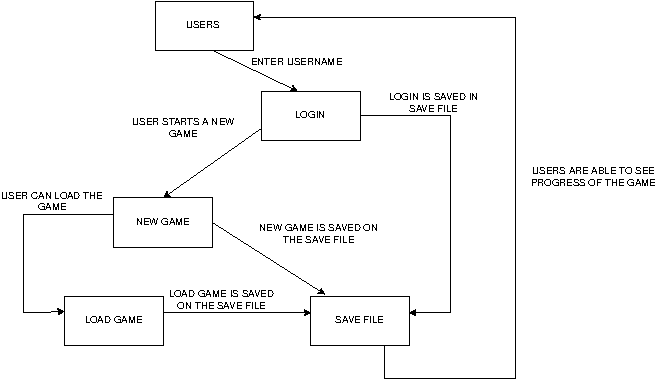
\includegraphics[scale=1,page=1]{2DGAME.drawio-crop.pdf}
\newpage
\section{Implementation}%
\label{sec:impl}
Our implementation will be completed in the Lua language and the love game
engine. We chose these tools as:
\begin{itemize}
	\item Lua is a small and simple language to learn. Being similar to python while
	      having many differing uses from python
	\item Love is a simple game engine, focusing in on 2d game development and
	      having a small and simple interface while still being able to express
	      larger and more complex games
\end{itemize}

%% TODO
We will be using git and github for our code management
\section{Testing}%
\label{sec:test}
Testing will mainly consist of unit testing. This allows us to test all of our
functions in isolation and check that we do not break compatability within
revisions.
%% TODO: Take user requrements and discuss how we would test them.
%% we can also use the design senarios

This will be followed by integration testing and then eventually user testing
\newpage
\section{Critical Analysis}%
\label{sec:anal}

\subsection{Leadership}%
\label{subsec:leadership}
Our methodology is Scrum. This will involve us assiging tasks into week long
sprints. These tasks will be tracked on a Kanban board hosted on github

We will have the roles of A scrum master and then scrum workers. The former will
delegate the tasks and monitor the progress of these tasks, with how these tasks
progressing being decided at the end of the sprint during our next meeting.

The Scrum master will be voted in during our weekly meetings. Everyone will have
a chance too but people will submit themselves. If no one does then we will
select the next person to not be scrum leader.

\subsection{Monitoring}%
\label{subsec:mon}
All tasks will be out on a monitoring board with a SCRUM Master monitoring progress throughout the week
Tasks are assigned at the beginning of each week.
As tasks are finished they will be move into a different section of the monitoring board
If a task is not finished during a sprint, then either more people will be assigned to it, it will get continued over to the next week or it will be reassigned to someone else

\subsection{Conflict resolution}%
\label{subsec:cres}

If a conflict of opinion comes into being. Then we will discuss this first in
our online communication channels.
If it does not resolve there then we will move this to a meeting, after
discussion with the entire group we will vote on it. A majority vote will be
taken.
If that fails to resolve the issue we will seek mediation from a third party

\subsubsection{Case study}
When deciding for this project we had mulitple projects we wanted to do.
This was not completed during our first session and we had a split between an
image sharing app and this 2d game.
We discussed this over our discord server and decided this would be better to
discuss in person.
During this in person meeting we wrote up the pros and cons of each, listing out
the technologies and the interesting sections of the problems. and finally came
to a vote. This process of multiple discussions was simple yet effective
%% TODO
%% add examples we have had disagreements
\end{document}
